%% Figure: Takens tau sensitivity sweep
%% Data source: data/output/heliosphere/ablations/takens_tau_sweep.json
%% Experiment: E-240  |  Claim: C-1633
%%
%% 5 methods: gradient baseline + CD at tau=1,2,5,10 minutes
%% Metrics: Precision, Recall, F1
%% THEMIS-A Staples+2020 catalog, 2016-08-29 to 2016-09-05, 224 events
\documentclass[tikz,border=4pt]{standalone}
\usepackage{pgfplots}
\usepackage{pgfplotstable}
\pgfplotsset{compat=1.18}
\usepackage{xcolor}

%% Okabe-Ito colorblind-safe palette
\definecolor{OIorange}{RGB}{230,159,0}
\definecolor{OIskyblue}{RGB}{86,180,233}
\definecolor{OIblue}{RGB}{0,114,178}
\definecolor{OIgreen}{RGB}{0,158,115}
\definecolor{OIgray}{RGB}{153,153,153}

\begin{document}
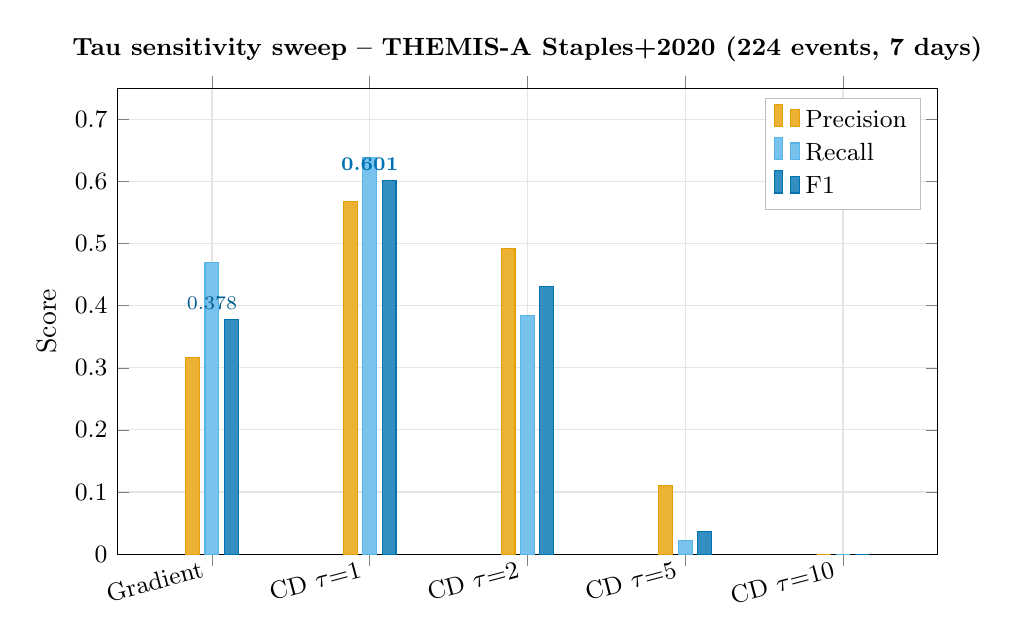
\begin{tikzpicture}
\begin{axis}[
    ybar,
    bar width=5pt,
    width=12cm,
    height=7.5cm,
    enlarge x limits=0.15,
    ylabel={Score},
    ymin=0, ymax=0.75,
    ytick={0,0.1,0.2,0.3,0.4,0.5,0.6,0.7},
    yticklabel style={font=\small},
    symbolic x coords={Gradient, {CD $\tau$=1}, {CD $\tau$=2}, {CD $\tau$=5}, {CD $\tau$=10}},
    xtick=data,
    xticklabel style={font=\small, rotate=15, anchor=east},
    legend style={at={(0.98,0.98)}, anchor=north east, font=\small,
                  draw=gray!50, fill=white},
    legend cell align=left,
    grid=major,
    grid style={gray!20},
    tick label style={font=\small},
    title style={font=\small\bfseries},
    title={Tau sensitivity sweep -- THEMIS-A Staples+2020 (224 events, 7 days)},
]

%% Precision bars
\addplot[fill=OIorange!80, draw=OIorange] coordinates {
    (Gradient,         0.317)
    ({CD $\tau$=1},    0.567)
    ({CD $\tau$=2},    0.492)
    ({CD $\tau$=5},    0.111)
    ({CD $\tau$=10},   0.000)
};
\addlegendentry{Precision}

%% Recall bars
\addplot[fill=OIskyblue!80, draw=OIskyblue] coordinates {
    (Gradient,         0.469)
    ({CD $\tau$=1},    0.638)
    ({CD $\tau$=2},    0.384)
    ({CD $\tau$=5},    0.022)
    ({CD $\tau$=10},   0.000)
};
\addlegendentry{Recall}

%% F1 bars
\addplot[fill=OIblue!80, draw=OIblue] coordinates {
    (Gradient,         0.378)
    ({CD $\tau$=1},    0.601)
    ({CD $\tau$=2},    0.431)
    ({CD $\tau$=5},    0.037)
    ({CD $\tau$=10},   0.000)
};
\addlegendentry{F1}

%% Annotate best CD F1
\node[font=\scriptsize\bfseries, text=OIblue, above] at
    (axis cs:{CD $\tau$=1}, 0.601) {0.601};

%% Annotate gradient F1 for comparison
\node[font=\scriptsize, text=OIblue!80!black, above] at
    (axis cs:Gradient, 0.378) {0.378};

\end{axis}
\end{tikzpicture}
\end{document}
